\documentclass[12pt]{article}
\usepackage{graphicx} % For including images/logo
\usepackage{geometry} % For custom margins
\usepackage{fancyhdr} % For custom headers/footers
\usepackage{titling}  % For custom title formatting
\usepackage{amsmath}  % For advanced math formatting
\usepackage{amssymb}  % For additional math symbols
\usepackage{enumitem} % For custom enumeration
\usepackage{xcolor}   % For text coloring
\usepackage{circuitikz}
\usepackage{animate}
% Set margins
\geometry{a4paper, margin=1in}

% Title, name, and date
\title{\textbf{EE1060 - DETT GROUP QUIZ 2}}
\author{EE24BTECH11012 - Bhavanisankar G S}
\date{\today}

% Add logo to the title
\pretitle{%
    \begin{center}
    
\includegraphics[width=0.5\textwidth]{figs/IITH.png} \\ % Replace with your logo file
    \vspace{1cm} % Adjust spacing as needed
    \LARGE
}
\posttitle{\end{center}}
\begin{document}

% First page with title, name, date, and logo
\maketitle
\thispagestyle{empty} % Remove page number from the first page

\newpage
\tableofcontents
\newpage

\section{\textbf{What is convolution ?}}

Convolution is a mathematical operation on two functions, $f$ and $g$, as the integral of the product of the two functions after one is reflected about the y-axis and shifted, i.e., If we are convolving a signal with a kernel, at each time $t$, we are sliding the kernel over the signal and computing how much they overlap. This is useful in various fields of study like finding the system response given the impulse response, signal processing and in probability.\\
Given two functions $f(x)$ and $g(x)$, convolution of the two signals, \\
\begin{align}
	x(t) &= f(t) * g(t) \\
	     &= \int_{-\infty}^{\infty} f(\tau) g(t - \tau) d \tau \label{eq:conv}
\end{align}
Some properties of convolution : \\
\begin{enumerate}
\item \textbf{Commutativity} : 
\begin{align*}
f(t) * g(t) &= g(t) * f(t)
\end{align*}
\item \textbf{Distributivity} :
\begin{align*}
f(t) * [g(t) + h(t)] &= [f(t) * g(t)] + [f(t) * h(t)] 
\end{align*}
\item \textbf{Associativity} :
\begin{align*}
f(t) * [g(t) * h(t)] &= [f(t) * g(t)] * h(t)
\end{align*}
\item \textbf{Time shifting property} :
If we are given $y(t) = x_1 (t) * x_2 (t)$, then
\begin{align*}
	x_1(t) * x_2(t - T) &= y(t - T) \\
	x_1(t - T) * x_2(t) &= y(t - T) \\
	x_1(t - T_1) * x_2(t - T_2) &= y(t - T_1 - T_2)
\end{align*}
\item \textbf{Width property} :
If the duration of signals $f(t)$ and $g(t)$ are $T_1$ and $T_2$ respectively, then the duration of signal convolving $f(t)$ and $g(t)$ is equal to $T_1 + T_2$
\end{enumerate}

\section{Convolution of sinc function}

Given kernel, 
\[
h(t) =
\begin{cases}
1, & \text{for } -T \leq t \leq T \\
0, & \text{otherwise}
\end{cases}
\]
and the function 
\begin{align*}
f(t) &= sinc(t) \\
     &= \frac{sint}{t}
\end{align*}
Let $y(t) = x(t) * f(t)$, then
\begin{align*}
	y(t) &= h(t) * f(t) \\
             &= f(t) * h(t) \\
             &= \int_{-\infty}^{\infty} f(\tau) h(t - \tau) d \tau \\
\end{align*}
\[
h(t - \tau) =
\begin{cases}
1, & \text{for } -T \leq t - \tau \leq T \\
0, & \text{otherwise}
\end{cases}
\]
\[
h(t - \tau) =
\begin{cases}
1, & \text{for } \tau - T \leq t \leq \tau + T \\
0, & \text{otherwise}
\end{cases}
\]
Therefore, the convolution becomes, 
\begin{align*}
	y(t) &= \int_{t - T}^{t + T} \frac{sin(\tau)}{\tau} * 1 d\tau \\
	y(t) &= \int_{t - T}^{t + T} \frac{sin(\tau)}{\tau} d\tau
\end{align*}
This integration can be numerically computed and can be seen to be the following - \\
\begin{figure}[!ht]
    \centering
    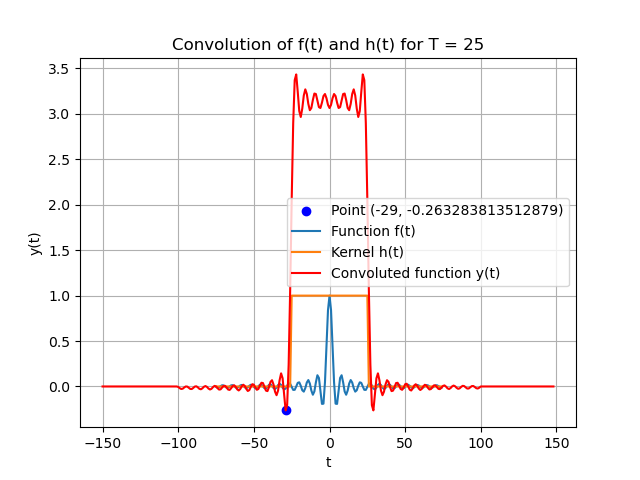
\includegraphics[width=0.6\textwidth]{figs/Conv_sinc.png}
    \caption{T = 25}
    \label{fig:conv_sinc}
\end{figure}
\newpage
For different values of T, the change in $y(t)$ is depicted in the following - \\
\begin{figure}[h]
    \centering
    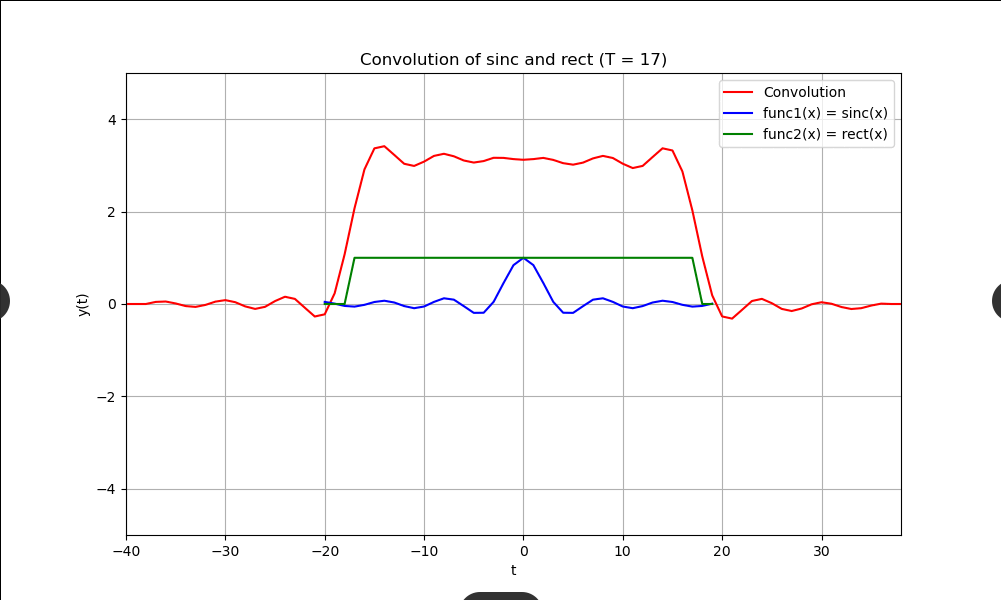
\includegraphics[width=0.6\textwidth]{figs/con1.png}
    \caption{T = 17}
    \label{fig:conv_sinc}
\end{figure}
\begin{figure}[h]
    \centering
    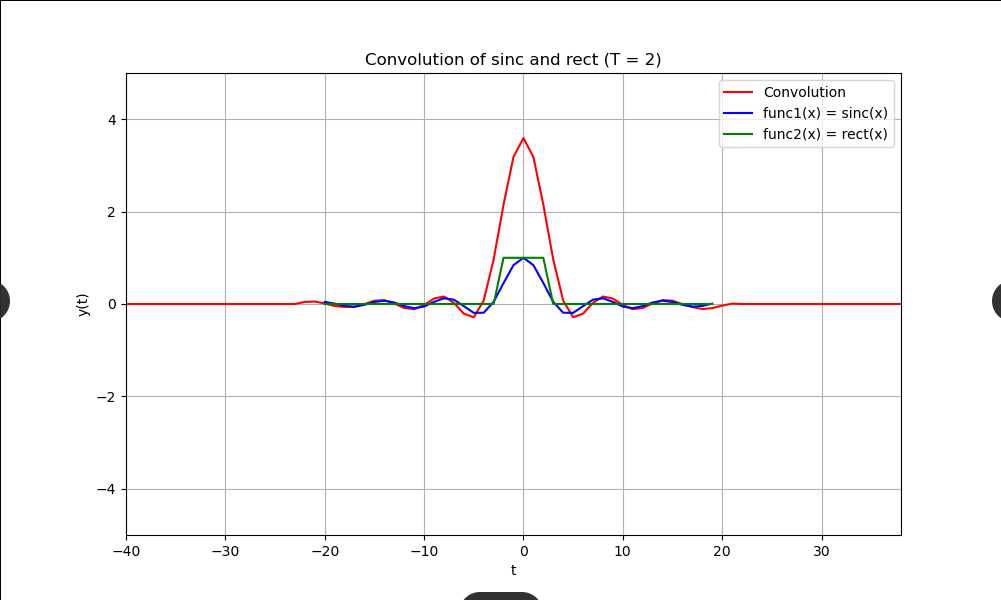
\includegraphics[width=0.6\textwidth]{figs/con2.png}
    \caption{T = 2}
    \label{fig:conv_sinc}
\end{figure}
\begin{figure}[h]
    \centering
    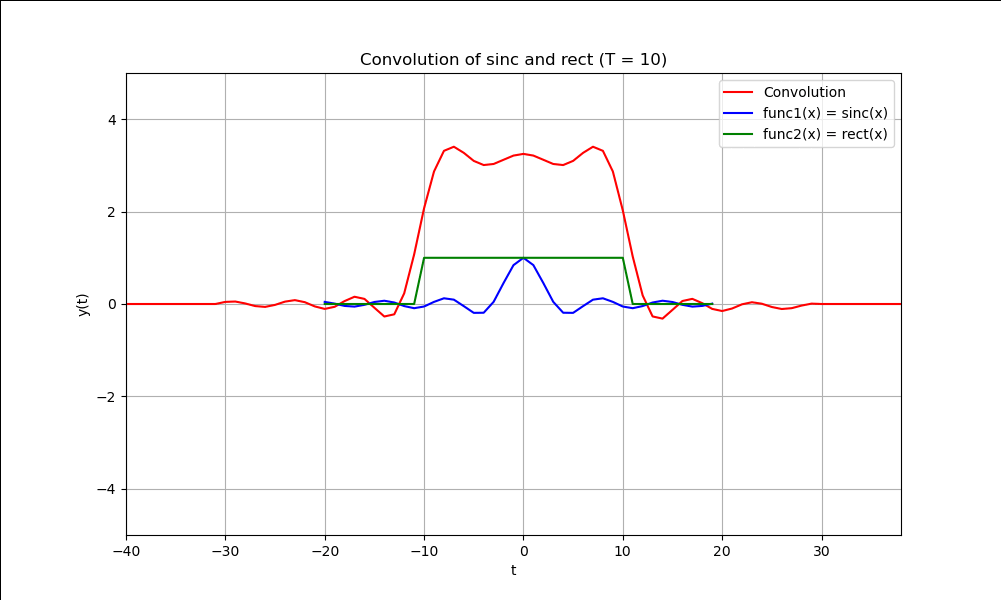
\includegraphics[width=0.6\textwidth]{figs/con3.png}
    \caption{T = 10}
    \label{fig:conv_sinc}
\end{figure}
\begin{figure}[h]
    \centering
    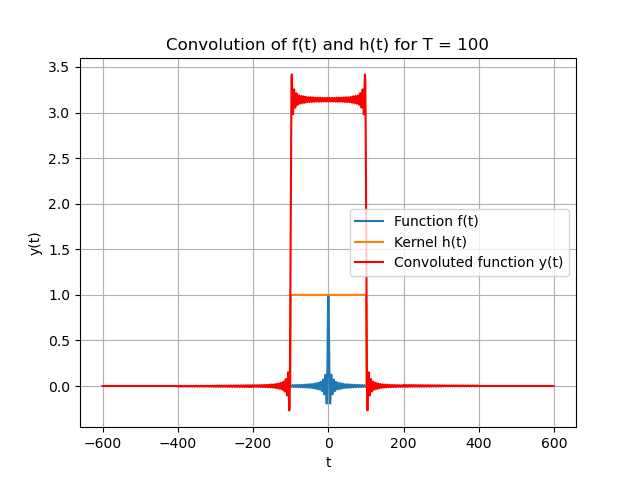
\includegraphics[width=0.6\textwidth]{figs/con4.png}
    \caption{T = 100}
    \label{fig:conv_sinc}
\end{figure}
\begin{figure}[h]
    \centering
    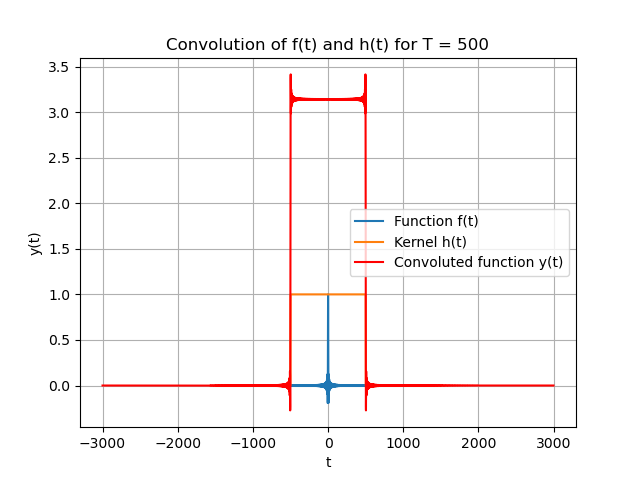
\includegraphics[width=0.6\textwidth]{figs/con5.png}
    \caption{T = 500}
    \label{fig:conv_sinc}
\end{figure}
\newpage
It can be seen that as $T$ increases, $y(t)$ becomes more square.

\newpage
\subsection{Considering the kernel for $t>0$}
The response of the system for different values of $T$ are as follows - \\
\begin{figure}[h]
    \centering
    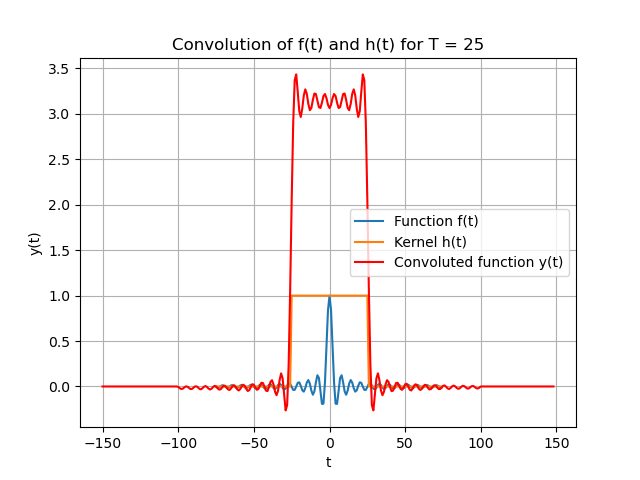
\includegraphics[width=0.6\textwidth]{figs/conv_sinc.png}
    \caption{T = 25}
    \label{fig:conv_sinc}
\end{figure}
\begin{figure}[h]
    \centering
    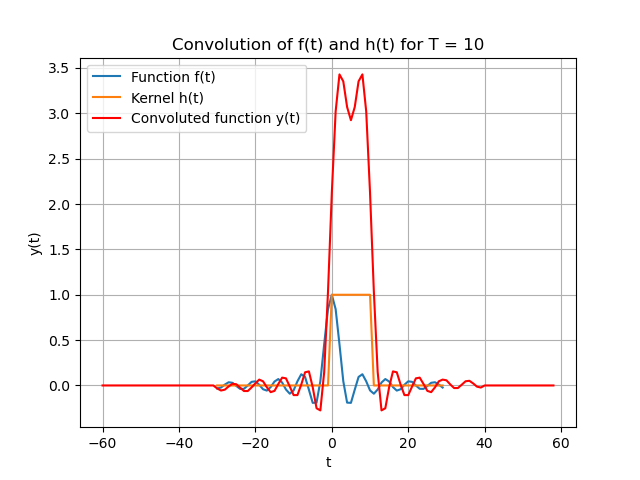
\includegraphics[width=0.6\textwidth]{figs/con6.png}
    \caption{T = 10}
    \label{fig:conv_sinc}
\end{figure}
\begin{figure}[h]
    \centering
    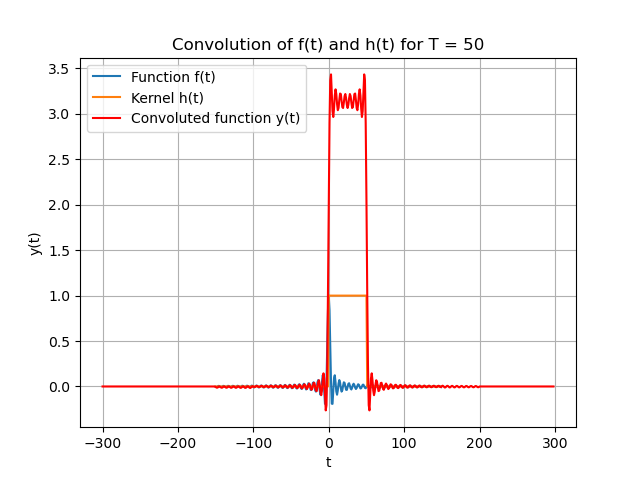
\includegraphics[width=0.6\textwidth]{figs/con7.png}
    \caption{T = 50}
    \label{fig:conv_sinc}
\end{figure}
\begin{figure}[h]
    \centering
    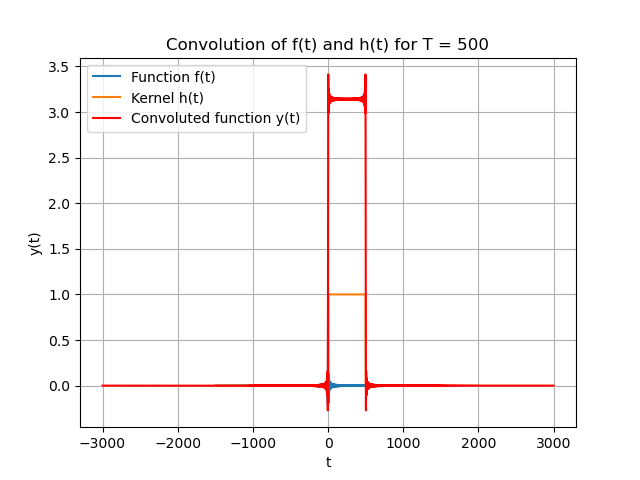
\includegraphics[width=0.6\textwidth]{figs/con8.png}
    \caption{T = 500}
    \label{fig:conv_sinc}
\end{figure}
It can be seen that the width of the convolution becomes half and it becomes shifted to the right.
\newpage

\subsection{Shifting the kernel by $t_{0}$}
Shifting of kernel means moving the kernel to the left or right by an amount, i.e., if the given kernel is shifted by an amount $t_0$, then it becomes, 
\[
h(t) =
\begin{cases}
1, & \text{for } -T \leq t-t_0 \leq T \\
0, & \text{otherwise}
\end{cases}
\]
\[
h(t) =
\begin{cases}
1, & \text{for } -T+t_0 \leq t \leq T+t_0 \\
0, & \text{otherwise}
\end{cases}
\]
If we are convolving a signal with the kernel, at each time $t$, we are sliding the kernel over the signal and computing how much they overlap. So, when we shift the kernel by $t_0$, we are changing when the kernel has its maximum influence.
This can physically mean applying a response $t_0$ time units early (or) $t_0$ time units late depending upon the sign of $t_0$, i.e., if $t_0 > 0$, the response is delayed and is advanced for $t_0 < 0$. This results in the convoluted signal also to be shifted by the same amount, as in figures \ref{fig:rshift} and \ref{fig:lshift} - 
\begin{figure*}[!htb]
    {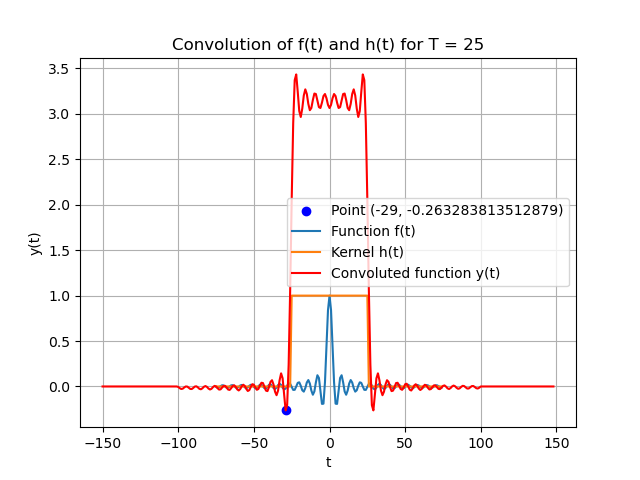
\includegraphics[ width=0.40\textwidth]{figs/Conv_sinc.png}}
    \hspace{\fill}
    {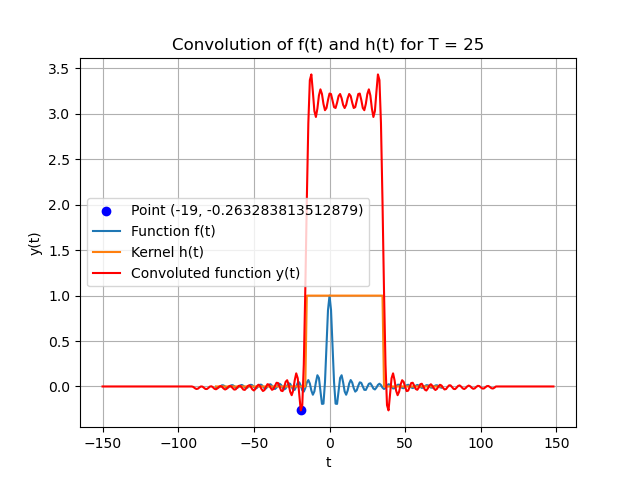
\includegraphics[ width=0.40\textwidth]{figs/conv_shift.png}}
    \hspace{\fill}\\
    \caption{Shifting toward right}
    \label{fig:rshift}
\end{figure*}
\begin{figure*}[!htb]
    {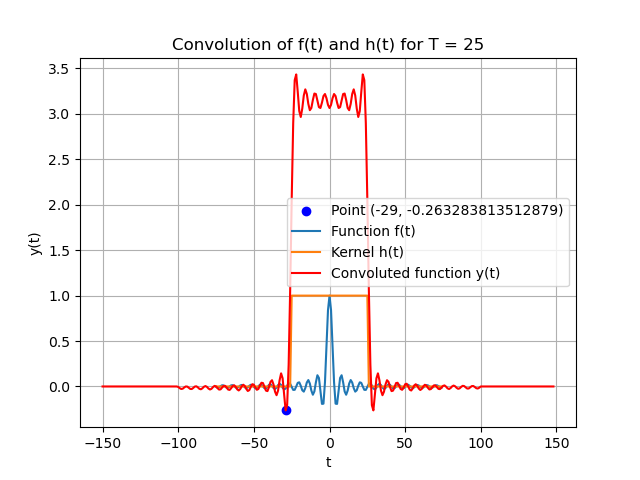
\includegraphics[ width=0.40\textwidth]{figs/Conv_sinc.png}}
    \hspace{\fill}
    {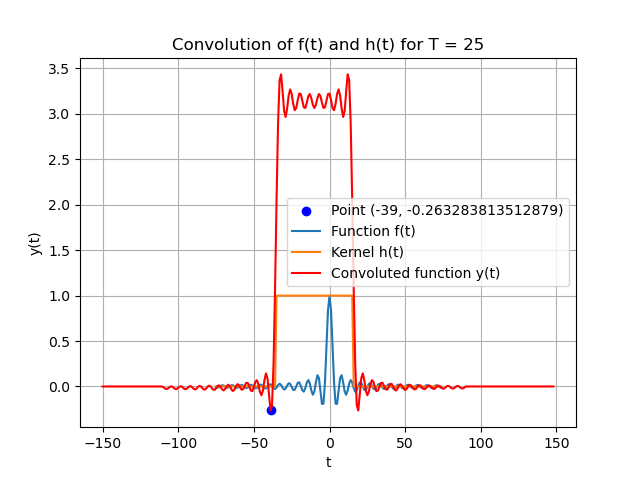
\includegraphics[ width=0.40\textwidth]{figs/conv_left.png}}
    \hspace{\fill}\\
    \caption{Shifting toward left}
    \label{fig:lshift}
\end{figure*}
Shifting of the kernel by 10 units results in shifting of convoluted function by 10 units.
\newpage
\section{Significance of time-shift}
\begin{enumerate}
\item In time-delayed systems, a positive shift ($t_0$) means that the system responds later to changes in the input. This can cause the system to react too slowly, which may lead to oscillations or instabilities in feedback systems, especially if the system relies on feedback loops (like in control systems or biological systems).
\item A negative shift ($t<0$) might result in the system anticipating the input and responding before it occurs. This could cause overreaction or instability if the system is not designed to handle anticipatory behavior.
\item In devices like thermostat, the system may respond to temperature changes with a delay because of the time it takes to heat/cool the room. By shifting of kernel, if the delay becomes too large, then the system might not be able to track the input accurately, leading to instability (or) oscillations.
\item In the context of signal processing, shifting the kernel corresponds to a phase shift in the signal, e.g., in delay filters, the impulse response can be delayed.
\item In biological systems, time delays are common in processes like hormonal responses, neural signals, or metabolic pathways. Shifting the kernel models how these systems react over time. For example, the delayed release of insulin after glucose intake could be modeled using a time-shifted kernel.

\end{enumerate}
\end{document}


	     
